\documentclass[12pt]{article}

\RequirePackage{amsmath}
\RequirePackage{amsthm}
\RequirePackage{amssymb}
\RequirePackage[mathscr]{eucal}
\RequirePackage{mathtools}
\RequirePackage{etoolbox}

\usepackage[red]{zhoucx-notation}

% correct bad hyphenation here
\hyphenation{op-tical net-works semi-conduc-tor}

\renewcommand{\qedsymbol}{\hfill\rule{2mm}{2mm}}

\pagestyle{fancy}
\fancyhf{}
\setlength{\headheight}{15pt}
\rhead{\textsf{Chapter 33, Sequential Data}}
\lhead{\textsf{Chenxi Zhou}}
\renewcommand{\headrulewidth}{1pt}
\cfoot{\thepage}

\newcommand{\titlebox}[4]{
\begin{tcolorbox}[colback = blue!5!white!95, colframe = blue!70!black
% colback = yellow!30!white, colframe = yellow!70!black 
]
  \noindent \textbf{ #1 } \hfill \textit{#2} 
  \begin{center}
  	 \LARGE{\textbf{#3}}
  \end{center}
\textbf{Chapter:} \textit{#4} \hfill \textbf{Prepared by:} \textit{Chenxi Zhou}
\end{tcolorbox}
}

\begin{document}

\titlebox{Notes on Statistical and Machine Learning}{}{Sequential Data}{33}
\thispagestyle{plain}

\vspace{10pt}

This note is prepared based on \textit{Chapter 13, Sequential Data} in \textcite{Bishop2016-tm}. 

\section*{I. Introduction}

\begin{enumerate}[label=\textbf{\arabic*.}]

	\item \textbf{Sequential Data:} We consider sequential data in this chapter, where data are not independent any more and but may come in a certain order and have correlation among them. 
	
	\textit{Examples:}
	\begin{itemize}
		\item The rainfall measurements on successive days at a particular location; 
		\item The daily values of a currency exchange rate; 
		\item The sequence of nucleotide base pairs along a strand of DNA; 
		\item The sequence of characters in an English sentence. 
	\end{itemize}
	
	\item \textbf{Stationary and Non-stationary Data:} 
	\begin{enumerate}
		\item \textit{Stationary Data:} In the stationary case, the data evolves in time, but the distribution from which it is generated remains the same; 
		\item \textit{Non-stationary Data:} For the non-stationary case, the generative distribution itself is evolving with time. 
	\end{enumerate}
	\textit{Remark.} We focus on the stationary case. 

\end{enumerate}


\section*{II. Markov Model}

\begin{enumerate}[label=\textbf{\arabic*.}]

	\item \textbf{Motivation:} 
	\begin{enumerate}
		\item We expect that \emph{recent} observations are likely to be more informative than more historical observations in predicting future values; 
		\item It would be \emph{impractical} to consider a general dependence of future observations on \emph{all} previous observations. 
	\end{enumerate}
	Hence, we consider \emph{Markov models} in which we assume that future predictions are independent of all but the most recent observations. 
	
	\item \textbf{General Product Rule in Probability:} Let $X_1, X_2, \cdots, X_n$ be a sequence of data. Their joint density function can be expressed as 
	\begin{align}\label{eq-product-rule}
		f_{X_1, X_2, \cdots, X_n} \parens{x_1, x_2, \cdots, x_n} = f_{X_1} \parens{x_1} \prod_{i=2}^n f_{X_i \,\vert\, X_{i-1}, \cdots, X_{1}} \parens{x_i \,\vert\, x_{i-1}, \cdots, x_1}, 
	\end{align}
	using the product rule. 
	
	\item \textbf{First-order Markov Model:} If we assume that each of the conditional distributions on the right-hand side of \eqref{eq-product-rule} is independent of all previous observations except the most recent, we obtain the \emph{first-order Markov model}. 
	
	In other words, the joint density function of $X_1, X_2, \cdots, X_n$ in the first-order Markov chain is factored as 
	\begin{align}
		f_{X_1, X_2, \cdots, X_n} \parens{x_1, x_2, \cdots, x_n} = f_{X_1} \parens{x_1} \prod_{i=2}^n f_{X_i \,\vert\, X_{i-1}} \parens{x_i \,\vert\, x_{i-1}}. 
	\end{align}
	
	\textit{Remark 1.} Under the first-order Markov model assumption, the conditional distribution for the $i$-th observation, given all observations up to time $i$, is 
	\begin{align*}
		f_{X_i \,\vert\, X_{i-1}, \cdots, X_{1}} \parens{x_i \,\vert\, x_{i-1}, x_{i-2}, \cdots, x_1} = f_{X_i \,\vert\, X_{i-1}} \parens{x_i \,\vert\, x_{i-1}}, 
	\end{align*}
	for all $i = 2, 3, \cdots, n$. 
	
	\textit{Remark 2.} If we use a first-order Markov model to predict the next observation in a sequence, the distribution of predictions depends only on the value of the immediately preceding observation and is independent of all earlier observations. 
	
	\item \textbf{Higher-order Markov Model:} If we assume that the current observation depends the past few observations, we obtain the higher-order Markov model. 
	
	For example, the density function of $X_1, X_2, \cdots, X_n$ under the second-order Markov model can be factored as 
	\begin{align*}
		f_{X_1, X_2, \cdots, X_n} \parens{x_1, x_2, \cdots, x_n} = f_{X_1} \parens{x_1} f_{X_2 \,\vert\, X_1} \parens{x_2 \,\vert\, x_1} \prod_{i=3}^n f_{X_{i} \,\vert\, X_{i-1}, X_{i-2}} \parens{x_i \,\vert\, x_{i-1}, x_{i-2}}, 
	\end{align*}
	where each observation is influenced by two previous observations. 
	
	\item \textbf{Model Complexity of $m$-th Order Markov Model:} Suppose the observation are discrete random variables having $K$ states. 
	\begin{enumerate}
		\item In a first-order Markov model, the conditional distribution $f_{X_i \,\vert\, X_{i-1}}$ is specified by a set of $K - 1$ parameters for each of the $K$ states of $X_{i-1}$. In total, we have $K \parens{K - 1}$ parameters in the model. 
		
		\item Consider an $m$-th order Markov chain where the joint density function is built up from conditionals 
		\begin{align*}
			f_{X_i \,\vert\, X_{i-1}, X_{i-2}, \cdots, X_{i-m}}. 
		\end{align*}
		If the conditional distributions are represented by general conditional probability tables, then the number of parameters in such a model will have $\calO \parens{K^{m}}$ parameters. 
		
		\textit{Remark.} Because the number of parameters grows exponentially with $m$, it will often render this approach \emph{impractical} for larger values of $m$. 
	\end{enumerate}
	
	\item \textbf{State-Space Model:} For each observation $X_i$ that is observed at time $i$, we introduce the corresponding latent variable $Z_i$ (which may be of different type or dimensionality to the observed variable) and assume these latent variables form a Markov chain, which gives rise to a \emph{state-space model}. A diagram of the state-space model is shown in Figure \ref{fig-state-space}. 
	
	\begin{figure}[h]
		\centering
		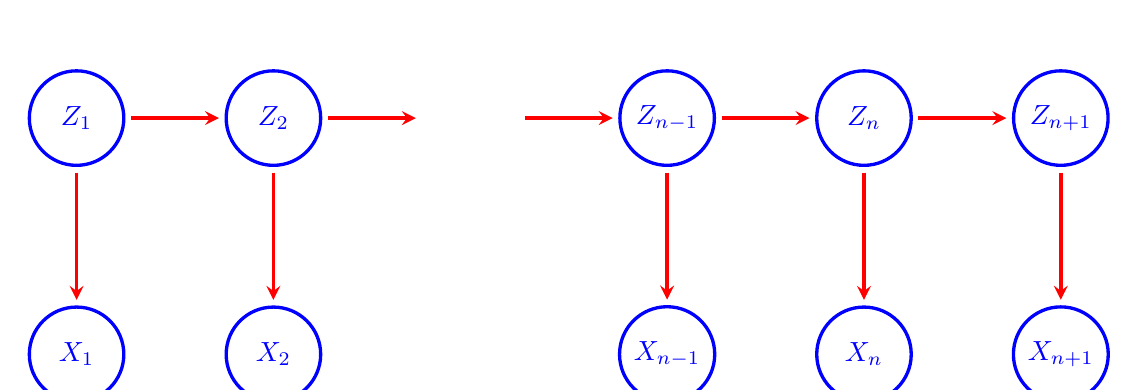
\begin{tikzpicture}
			\node[draw,circle,minimum size=1.2cm,minimum width=1.2cm,color=blue,very thick] (p1) at (0,2){$Z_1$};
			\node[draw,circle,minimum size=1.2cm,minimum width=1.2cm,color=blue,very thick] (p2) at (2.5,2){$Z_2$};
			\node[draw,circle,minimum size=1.2cm,minimum width=1.2cm,color=white,very thick] (p3) at (5,2){$\cdots$};
			\node[draw,circle,minimum size=1.2cm,minimum width=1.2cm,color=blue,very thick] (p4) at (7.5,2){$Z_{n-1}$};
			\node[draw,circle,minimum size=1.2cm,minimum width=1.2cm,color=blue,very thick] (p5) at (10,2){$Z_{n}$};
			\node[draw,circle,minimum size=1.2cm,minimum width=1.2cm,color=blue,very thick] (p6) at (12.5,2){$Z_{n+1}$}; 
			
			\node[draw,circle,minimum size=1.2cm,minimum width=1.2cm,color=blue,very thick] (p7) at (0,-1){$X_1$};
			\node[draw,circle,minimum size=1.2cm,minimum width=1.2cm,color=blue,very thick] (p8) at (2.5,-1){$X_2$};
			\node[draw,circle,minimum size=1.2cm,minimum width=1.2cm,color=white,very thick] (p9) at (5,-1){$\cdots$};
			\node[draw,circle,minimum size=1.2cm,minimum width=1.2cm,color=blue,very thick] (p10) at (7.5,-1){$X_{n-1}$};
			\node[draw,circle,minimum size=1.2cm,minimum width=1.2cm,color=blue,very thick] (p11) at (10,-1){$X_{n}$};
			\node[draw,circle,minimum size=1.2cm,minimum width=1.2cm,color=blue,very thick] (p12) at (12.5,-1){$X_{n+1}$}; 
			
			\draw (p1) edge [->,>=stealth,shorten <=2pt, shorten >=2pt, very thick, color = red] (p2); 
			\draw (p2) edge [->,>=stealth,shorten <=2pt, shorten >=2pt, very thick, color = red] (p3); 
			\draw (p3) edge [->,>=stealth,shorten <=2pt, shorten >=2pt, very thick, color = red] (p4); 
			\draw (p4) edge [->,>=stealth,shorten <=2pt, shorten >=2pt, very thick, color = red] (p5); 
			\draw (p5) edge [->,>=stealth,shorten <=2pt, shorten >=2pt, very thick, color = red] (p6); 
			
			\draw (p1) edge [->,>=stealth,shorten <=2pt, shorten >=2pt, very thick, color = red] (p7); 
			\draw (p2) edge [->,>=stealth,shorten <=2pt, shorten >=2pt, very thick, color = red] (p8); 
			\draw (p4) edge [->,>=stealth,shorten <=2pt, shorten >=2pt, very thick, color = red] (p10); 
			\draw (p5) edge [->,>=stealth,shorten <=2pt, shorten >=2pt, very thick, color = red] (p11); 
			\draw (p6) edge [->,>=stealth,shorten <=2pt, shorten >=2pt, very thick, color = red] (p12); 
		\end{tikzpicture}
		\captionsetup{width=.7\linewidth}
		\caption{Diagram associated with the state-space model.}
		\label{fig-state-space}
	\end{figure}
	
	The join density function of $X_1, X_2, \cdots, X_n, Z_1, Z_2, \cdots, Z_n$ is given by 
	\begin{align*}
		& \, f_{X_1, \cdots, X_n, Z_1, \cdots, Z_n} \parens{x_1, \cdots, x_n, z_1, \cdots, z_n} \\ 
		& \qquad \qquad = f_{Z_1} \parens{z_1} \bracks[\Bigg]{\prod_{i=2}^n f_{Z_i \vert Z_{i-1}} \parens{z_i \,\vert\, z_{i-1}}} \bracks[\Bigg]{\prod_{i=1}^n f_{X_i \vert Z_i} \parens{x_i \,\vert\, z_{i}}}.  
	\end{align*}
	
	\textit{Remark 1.} In such a state-space model, $Z_{i-1}$ and $Z_{i+1}$ are independent given $Z_i$, for all $i = 2, 3, \cdots, n$. 
	
	\textit{Remark 2.} There is always a path connecting any two observed variables $X_i$ and $X_j$ via the latent variables, and that this path is never blocked. 
	
\end{enumerate}


\section*{III. Hidden Markov Models}

\begin{enumerate}[label=\textbf{\arabic*.}]
	
	\item \textbf{Hidden Markov Models:} If the latent variables in the state-space model are discrete random variables, we obtain the \emph{hidden Markov model}. 
	
	\item \textbf{Homogeneity Assumption:} We assume that all parameters in the model (see below) are independent of the time stamp. In other words, for all $i \neq j$, 
	\begin{itemize}
		\item the parameters appearing in $f_{Z_i \vert Z_{i-1}}$ are identical to those appearing in $f_{Z_j \vert Z_{j-1}}$, and 
		\item the parameters appearing in $f_{X_i \,\vert\, Z_{i}}$ are identical to those appearing in $f_{X_j \,\vert\, Z_{j}}$. 
	\end{itemize}
	
	\item \textbf{Model Specification --- Distribution of $Z_1$:} We assume that $Z_1$ follows a multinomial distribution with $K$ components and can take any values in $\braces{1, 2, \cdots, K}$. We introduce the following notation 
	\begin{align*}
		\widetilde{Z}_{1, k} = \begin{cases}
			1, & \, \text{ if } Z_1 = k, \\ 
			0, & \, \text{ otherwise}, 
		\end{cases}
	\end{align*}
	and let 
	\begin{align*}
		\widetilde{Z}_1 := \parens{\widetilde{Z}_{1,1}, \widetilde{Z}_{1,2}, \cdots, \widetilde{Z}_{1,K}} \in \Real^K. 
	\end{align*}
	
	Since the initial latent variable $Z_1$ does \emph{not} have a parent node, we consider its marginal distribution and let 
	\begin{align*}
		\pi_k := \Pr \parens{Z_1 = k} = \Pr \parens{\widetilde{Z}_{1,k} = 1}, \qquad \text{ for all } k = 1, 2, \cdots, K. 
	\end{align*}
	Note that $\pi_1, \pi_2, \cdots, \pi_K$ must satisfy 
	\begin{align*}
		\pi_k \ge 0 \qquad \text{ for all } k = 1, 2, \cdots, K
	\end{align*}
	and 
	\begin{align}\label{eq-constraint-pi}
		\sum_{k=1}^K \pi_k = 1. 
	\end{align}
	We let $\bpi := \parens{\pi_1, \pi_2, \cdots, \pi_K}^{\top} \in \Real^K$. 
	
	\textit{Remark.} Note that exactly one entry of $\widetilde{Z}_1$ is equal to 1 and all others are equal to 0. 
	
	\item \textbf{Model Specification --- Conditional Distribution of Latent Variables:} We assume that, conditional on $Z_{i-1}$, $Z_i$ follows a multinomial distribution with $K$ components, for all $i = 2, 3, \cdots$, and can take any values in $\sets{1, 2, \cdots, K}$. Similar to $\widetilde{Z}_1$, we introduce the following notation: conditional on $Z_{i-1}$, let 
	\begin{align*}
		\widetilde{Z}_{i,k} = \begin{cases}
			1, & \, \text{ if } Z_i = k, \\ 
			0, & \, \text{ otherwise}, 
		\end{cases} \qquad 
	\end{align*}
	for all $k = 1, 2, \cdots, K$ and $i = 2, 3, \cdots$, and collectively, let 
	\begin{align*}
		\widetilde{Z}_i := \parens{\widetilde{Z}_{i,1}, \widetilde{Z}_{i,2}, \cdots, \widetilde{Z}_{i,K}}, 
	\end{align*}
	for all $i = 2, 3, \cdots$. 
	
	Under the multinomial distribution assumption, the conditional distribution of $Z_i$, given $Z_{i-1}$, corresponds to a table of numbers, denoted by $\bA \in \Real^{K \times K}$, where 
	\begin{align*}
		A_{j, k} = & \, \Pr \parens{Z_{i} = k \,\vert\, Z_{i-1} = j} 
		= \Pr \parens{\widetilde{Z}_{i,k} = 1 \,\vert\, \widetilde{Z}_{i-1,j} = 1}, 
	\end{align*}
	for all $j, k = 1, 2, \cdots, K$. Note that $A_{j,k}$'s satisfy 
	\begin{align}\label{eq-transition-prob}
		A_{j,k} \ge 0 \qquad \text{ and } \qquad \sum_{k=1}^K A_{j,k} = 1. 
	\end{align}
	The elements of $\bA$, $A_{j,k}$'s, are called the \emph{transition probabilities}. 
	
%	The conditional distribution can be written explicitly as 
%	\begin{align}
%		p_{\bA} \parens{Z_i \,\vert\, Z_{i-1}} = \prod_{k=1}^K \prod_{j=1}^K A_{j,k} \indic_{\sets{Z_{n-1} = j, Z_n = k}}, 
%	\end{align}
%	for all $i = 2, 3, \cdots, n$. 
	
	\textit{Remark.} Due to the constraints in \eqref{eq-transition-prob}, the matrix $\bA$ has $K \parens{K-1}$ independent parameters. 
	
	\item \textbf{Model Specification --- Conditional Distribution of Observed Variables:} Conditioning on $Z_i = k$, we let the density function of $X_i$ be 
	\begin{align*}
		f_{X_i \vert Z_i = k} \parens{\,\cdot\, \vert\, \phi_k}, 
	\end{align*}
	where $\phi_k$ is a set of parameters governing the density function. Collectively, we write $\boldsymbol{\phi} := \parens{\phi_1, \phi_2, \cdots, \phi_K}$. 
	
	\item \textbf{Joint Density Function of Latent and Observed Variables:} Under the assumptions and notation above, the joint probability density function of the observed variables, $X_1, X_2, \cdots, X_n$, and the latent variables, $Z_1, Z_2, \cdots, Z_n$, is given by 
	\begin{align}
		& \, f_{X_1, \cdots, X_n, \widetilde{Z}_1, \cdots, \widetilde{Z}_n} \parens{x_1, x_2, \cdots, x_n, \tilde{\bz}_1, \tilde{\bz}_2, \cdots, \tilde{\bz}_n \,\vert\, \btheta} \nonumber \\ 
		& \qquad \qquad  = \bracks[\Bigg]{\prod_{k=1}^K \pi_k^{\tilde{z}_{1,k}}} \bracks[\Bigg]{\prod_{i=2}^n \prod_{k=1}^K \prod_{j=1}^K A_{j,k}^{\tilde{z}_{i-1,j} \tilde{z}_{i,k}} } \bracks[\Bigg]{\prod_{i=1}^n \prod_{k=1}^K \parens[\big]{f_{X_i \vert Z_i = k} \parens{x_i \vert\, \phi_k}}^{\tilde{z}_{i,k}}}, \label{eq-joint-pdf}
	\end{align}
	where $\btheta := \parens{\bA, \bpi, \boldsymbol{\phi}}$. 
	
	\textit{Remark 1.} We used the homogeneity assumption above; more explicitly, 
	\begin{itemize}
		\item all conditional distributions governing the latent variables share the same parameters $\bA$, and 
		\item all conditional distributions governing the observed variables share the same parameters $\phi_k$'s. 
	\end{itemize}
	These parameters only depends on the appropriate states but not the time stamps. 
	
	\textit{Remark 2.} The model here is tractable for a wide range of $f_{X_i \vert Z_i = k} \parens{\,\cdot\, \vert\, \phi_k}$ including discrete tables, Gaussians, mixtures of Gaussians, or even neural networks. 
	
	\item \textbf{Sampling from Hidden Markov Model:} We can obtain samples from a hidden Markov model as follows: 
	\begin{enumerate}
		\item Choose the initial latent variable $Z_1$ with probabilities governed by the parameters $\pi_1, \pi_2, \cdots, \pi_K$, and then sample the corresponding observation $X_1$; 
		\item Choose the state of the variable $Z_2$ according to the transition probabilities $\Pr \parens{Z_2 \,\vert\, Z_1}$ using $Z_1$: supposing $Z_1 = j$ for some $j \in \sets{1, 2, \cdots, K}$, we sample $Z_2$ according to probabilities $\parens{A_{j,1}, A_{j,2}, \cdots, A_{j,K}}$; 
		\item Once we know $Z_2$, we can draw a sample for $X_2$ and also sample the next latent variable $Z_3$ and so on. 
	\end{enumerate}
	
	\textit{Remark.} The sampling procedure outlined here is an example of \emph{ancestral sampling} for a directed graphical model. 
	
	\item \textbf{Difficulties in Parameter Estimation Using Maximum Likelihood:} Suppose the observed data are given as $\bX := \sets{x_1, x_2, \cdots, x_n}$ and the hidden data are given as $\widetilde{\bZ} := \sets{\widetilde{\bz}_1, \widetilde{\bz}_2, \cdots, \widetilde{\bz}_n}$. The likelihood function can be obtained by marginalizing \eqref{eq-joint-pdf} over the latent variables 
	\begin{align}\label{eq-likelihood-direct}
		L \parens{\btheta \,\vert\, \bX} = \sum_{\widetilde{\bZ}} f_{X_1, \cdots, X_n, \widetilde{Z}_1, \cdots, \widetilde{Z}_n} \parens{x_1, x_2, \cdots, x_n, \tilde{\bz}_1, \tilde{\bz}_2, \cdots, \tilde{\bz}_n \,\vert\, \btheta}. 
	\end{align}
	Direct maximization of $L$ above is intractable by noting that the summation in \eqref{eq-likelihood-direct} corresponds to summing over $K^n$ terms. 
	
	\item \textbf{EM Algorithm to Estimate $\btheta$ --- Overview:} We use the expectation-maximization (EM) algorithm to maximize the likelihood function in hidden Markov models. 
	
	The EM algorithm starts with some initial selection for the model parameters, which we denote by $\btheta^{\mathrm{old}}$. Then, 
	\begin{enumerate}
		\item in the E step, we take $\btheta^{\mathrm{old}}$ and find the conditional distribution of the latent variables $f \parens{\widetilde{\bZ} \,\vert\, \bX, \btheta^{\mathrm{old}}}$, using which we evaluate the expectation of the logarithm of the complete-data likelihood function; 
		\item in the M step, we maximize the expectation with respect to the parameters. 
	\end{enumerate}
	
	\item \textbf{EM Algorithm to Estimate $\btheta$ --- E Step:} With the current value of the parameters $\btheta^{\mathrm{old}}$, in the E step, we evaluate the expectation of the logarithm of the complete data likelihood function as a function of the parameters $\btheta$; that is, we compute 
	\begin{align}
		Q \parens{\btheta, \btheta^{\mathrm{old}}} := \sum_{\widetilde{\bZ}} f \parens{\widetilde{\bZ} \,\vert\, \bX, \btheta^{\mathrm{old}}} \log f \parens{\bX, \widetilde{\bZ} \,\vert\, \btheta}, 
	\end{align}
	where we omit the subscripts for density functions. Note that 
	\begin{align*}
		\log f \parens{\bX, \widetilde{\bZ} \,\vert\, \btheta} = & \, \sum_{k=1}^K \tilde{z}_{1,k} \log \pi_k + \sum_{i=2}^n \sum_{k=1}^K \sum_{j=1}^K \tilde{z}_{i-1,j} \tilde{z}_{i, k} \log A_{j, k} \\ 
		& \qquad + \sum_{i=1}^n \sum_{k=1}^K \tilde{z}_{i,k} \log f_{X_i \vert Z_i = k} \parens{x_i \,\vert\, \phi_k}. 
	\end{align*}
	Then, it can be shown that 
	\begin{align*}
		Q \parens{\btheta, \btheta^{\mathrm{old}}} = & \, \sum_{k=1}^K \gamma \parens{\widetilde{Z}_{1,k}} \log \pi_k + \sum_{i=2}^n \sum_{k=1}^K \sum_{j=1}^K \xi \parens{\widetilde{Z}_{i-1,j}, \widetilde{Z}_{i,k}} \log A_{j,k} \\ 
		& \qquad \qquad \qquad \qquad \quad + \sum_{i=1}^n \sum_{k=1}^K \gamma \parens{\widetilde{Z}_{i,k}} \log f_{X_i \vert Z_i = k} \parens{x_i \,\vert\, \phi_k}, 
	\end{align*}
	where 
	\begin{align*}
		\gamma \parens{\widetilde{Z}_{i,k}} = & \, \Pr \parens{\widetilde{Z}_{i,k} = 1 \,\vert\, \bX, \btheta^{\mathrm{old}}}, \\ 
		\xi \parens{\widetilde{Z}_{i-1,j}, \widetilde{Z}_{i,k}} = & \, \Pr \parens{\tilde{Z}_{i-1,j} = 1, \widetilde{Z}_{i,k} = 1 \,\vert\, \bX, \btheta^{\mathrm{old}}}. 
	\end{align*}
	
	\item \textbf{EM Algorithm to Estimate $\btheta$ --- M Step:} In the M step, we maximize $Q \parens{\,\cdot\,, \btheta^{\mathrm{old}}}$ with respect to the first argument by treating the quantities $\gamma \parens{\widetilde{Z}_{i,k}}$'s and $\xi \parens{\widetilde{Z}_{i-1,j}, \widetilde{Z}_{i,k}}$'s as known. Recall that $\btheta$ involves three parts, namely, $\bpi$, $\bA$, and $\boldsymbol{\phi}$. 
	\begin{enumerate}
		\item \textit{Maximizing Over $\bpi$:} Maximizing over $\bpi$ under the constraint $\sum_{k=1}^K \pi_k = 1$ yields 
		\begin{align*}
			\widehat{\pi}_k = \frac{\gamma \parens{\widetilde{Z}_{1,k}}}{\sum_{j=1}^K \gamma \parens{\widetilde{Z}_{1,j}}}, \qquad \text{ for all } k = 1, 2, \cdots, K. 
		\end{align*}
		
		\item \textit{Maximizing Over $\bA$:} Maximizing over $\bA$ under the constraint $\sum_{k=1}^K A_{j,k} = 1$, for all $j = 1, 2, \cdots, K$, yields 
		\begin{align*}
			\widehat{A}_{j,k} = \frac{\sum_{i=2}^n \xi \parens{\widetilde{Z}_{i-1,j}, \widetilde{Z}_{i,k}}}{\sum_{\ell=1}^K \sum_{i=2}^n \xi \parens{\widetilde{Z}_{i-1,j}, \widetilde{Z}_{i,\ell}}}, \qquad \text{ for all } j, k = 1, 2, \cdots, K. 
		\end{align*}
		
		\item \textit{Maximizing Over $\boldsymbol{\phi}$:} Maximizing over $\boldsymbol{\phi}$ is data dependent and depends on the specific form of the conditional density functions $p_{\phi_k}$'s. 
		
		For example, if $f_{X_i \vert Z_i = k} \parens{\,\cdot \,\vert\, \phi_k}$ is the density function of the normal distribution with mean $\bmu_k$ and covariance matrix $\bSigma_k$, maximizing $Q \parens{\,\cdot\,, \btheta^{\mathrm{old}}}$ with respect to $\bmu_k$ and $\bSigma_k$ yields the following estimators  
		\begin{align*}
			\widehat{\bmu}_k = & \, \frac{\sum_{i=1}^n \gamma \parens{\widetilde{Z}_{i,k}} x_i}{\sum_{i=1}^n \gamma \parens{\widetilde{Z}_{i,k}}}, \\ 
			\widehat{\bSigma}_k = & \, \frac{\sum_{i=1}^n \gamma \parens{\widetilde{Z}_{i,k}} \parens{x_i - \widehat{\bmu}_k} \parens{x_i - \widehat{\bmu}_k}^\top }{\sum_{i=1}^n \gamma \parens{\widetilde{Z}_{i,k}}}, 
		\end{align*}
		respectively, for all $k = 1, 2, \cdots, K$. 
		
%		\item \underline{Multinomial Conditional Distribution:} If $f_{X_i \vert Z_i = k} \parens{\,\cdot \,\vert\, \phi_k}$ is the probability mass function of the multinomial distribution with $M$ components and cell probabilities $\rho_{k,1}, \rho_{k,2}, \cdots, \rho_{k,M}$, i.e., 
%		\begin{align*}
%			p_{\phi_k} \parens{x} = \prod_{m=1}^M \rho_{k,m} \indic_{x = m}, 
%		\end{align*}
%		then, maximizing $Q \parens{\,\cdot\,, \btheta^{\mathrm{old}}}$ with respect to $\rho_{k,m}$'s yields the following maximizer 
%		\begin{align*}
%			\widehat{\brho}_{k,m} = \frac{\sum_{i=1}^n \gamma \parens{\widetilde{Z}_{i,k}} \indic_{X_i=m}}{\sum_{i=1}^n \gamma \parens{\widetilde{Z}_{i,k}}}, 
%		\end{align*}
%		for all $m = 1, 2, \cdots, M$. 
	\end{enumerate}
	
	\textit{Remark.} The parameters $\bpi$ and $\bA$ must be initialized in a way such that the constraints \eqref{eq-constraint-pi} and \eqref{eq-transition-prob} are satisfied. 
	
	Any elements of $\bpi$ or $\bA$ that are set to zero initially will remain zero in subsequent EM updates. 
	
%	\item \textbf{Evaluating $\gamma \parens{\widetilde{Z}_{i,k}}$'s and $\xi \parens{\widetilde{Z}_{i-1,j}, \widetilde{Z}_{i,k}}$'s --- Overview:} We derive the explicit formula for $\gamma \parens{\widetilde{Z}_{i,k}}$'s and $\xi \parens{\widetilde{Z}_{i-1,j}, \widetilde{Z}_{i,k}}$'s using 
%	\begin{itemize}
%		\item the sum and product rules of probability, and 
%		\item the conditional independence properties. 
%	\end{itemize}
%	Some remarks are the following: 
%	\begin{enumerate}
%		\item Evaluation of $\gamma \parens{\widetilde{Z}_{i,k}}$'s and $\xi \parens{\widetilde{Z}_{i-1,j}, \widetilde{Z}_{i,k}}$'s is independent of whether the observed variables are continuous or discrete. All we require is the values of the quantities $p_{\phi_k}$ for each $k$; 
%		\item We omit the explicit dependence on the model parameters $\btheta^{\mathrm{old}}$ because these fixed throughout in the E step. 
%	\end{enumerate}
%	
%	\item \textbf{Useful Conditional Independence Properties:} The following conditional independence properties are useful in deriving the formula for $\gamma \parens{\widetilde{Z}_{i,k}}$'s and $\xi \parens{\widetilde{Z}_{i-1,j}, \widetilde{Z}_{i,k}}$'s: 
%	\begin{enumerate}
%		\item $p \parens{X_1, X_2, \cdots, X_n \,\vert\, \widetilde{\bZ}_i} = p \parens{X_1, X_2, \cdots, X_i \,\vert\, \widetilde{\bZ}_i} \times p \parens{X_{i+1}, X_{i+2}, \cdots, X_n \,\vert\, \widetilde{\bZ}_i}$, 
%		\item $p \parens{X_1, X_2, \cdots, X_{i-1} \,\vert\, X_{i}, \widetilde{\bZ}_i} = p \parens{X_1, X_2, \cdots, X_{i-1} \,\vert\, \widetilde{\bZ}_i}$, 
%		\item $p \parens{X_1, X_2, \cdots, X_{i-1} \,\vert\, \widetilde{\bZ}_{i-1}, \widetilde{\bZ}_i} = p \parens{X_1, X_2, \cdots, X_{i-1} \,\vert\, \widetilde{\bZ}_{i-1}}$, 
%		\item $p \parens{X_{i+1}, X_{i+2}, \cdots, X_{n} \,\vert\, \widetilde{\bZ}_{i}, \widetilde{\bZ}_{i+1}} = p \parens{X_{i+1}, X_{i+2}, \cdots, X_{n} \,\vert\, \widetilde{\bZ}_{i+1}}$, 
%		\item $p \parens{X_{i+2}, \cdots, X_{n} \,\vert\, \widetilde{\bZ}_{i+1}, X_{i+1}} = p \parens{X_{i+2}, \cdots, X_{n} \,\vert\, \widetilde{\bZ}_{i+1}}$, 
%		\item $p \parens{X_{1}, X_{2}, \cdots, X_{n} \,\vert\, \widetilde{\bZ}_{i-1}, \widetilde{\bZ}_{i}} = p \parens{X_{1}, \cdots, X_{i-1} \,\vert\, \widetilde{\bZ}_{i-1}} \times p \parens{X_i \,\vert\, \widetilde{\bZ}_{i}} \times p \parens{X_{i+1}, \cdots, X_{n} \,\vert\, \widetilde{\bZ}_{i}}$, 
%		\item $p \parens{X_{i+1}, \,\vert\, X_1, \cdots, X_n, \widetilde{\bZ}_{i+1}} = p \parens{X_{i+1} \,\vert\, \widetilde{\bZ}_{i+1}}$, 
%		\item $p \parens{\widetilde{\bZ}_{n+1} \,\vert\, \widetilde{\bZ}_{n}, X_1, \cdots, X_{n}} = p \parens{\widetilde{\bZ}_{n+1} \,\vert\, \widetilde{\bZ}_{n}}$. 
%	\end{enumerate}
%	
%	\item \textbf{Evaluating $\gamma \parens{\widetilde{Z}_{i,k}}$:} By the definition, we have 
%	\begin{align*}
%		\gamma \parens{\widetilde{Z}_{i,k}} = \Pr \parens{\widetilde{Z}_{i,k} = 1 \,\vert\, X_1, \cdots, X_n} = \frac{p \parens{X_1, X_2, \cdots, X_n \,\vert\, \widetilde{Z}_{i,k} = 1} \Pr \parens{\widetilde{Z}_{i,k} = 1}}{p \parens{X_1, X_2, \cdots, X_n}} \\ 
%		= & \, 
%	\end{align*}
%
\end{enumerate}


\printbibliography

\end{document}
